% !TeX spellcheck = de_DE
\documentclass[a4paper,12pt]{article}
\usepackage[bahasa]{babel}
\usepackage{graphicx}
\graphicspath{ {./img/} }
\begin{document}
\title{Laporan Praktikum Statistika Pertemuan 7}
%\author{Aldzikri Dwijayanto Prathama \\ {\small 195410189}}
\author{Aldzikri Dwijayanto Prathama 
	\\195410189}
\makeatletter
\begin{titlepage}
	\begin{center}
		{\huge \bfseries \@title }\\[14ex]
		
\includegraphics[scale=.8]{logo}\\[4ex]
		{\large \@author}\\[20ex]
		{\large \bfseries {SEKOLAH TINGGI MANAJEMEN INFORMATIKA DAN KOMPUTER
				AKAKOM YOGYAKARTA}}
	\end{center}


%{\large \@date} 
\end{titlepage}
\makeatother
%\maketitle
\newpage
\section{Praktik}
\subsection{Tabel Kontigensi}
\subsubsection{Praktik 1}
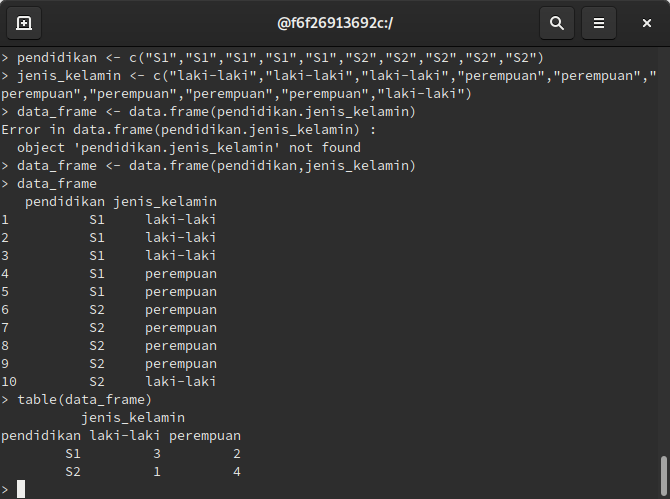
\includegraphics[width=\linewidth]{1}
\subsubsection{Praktik 2}
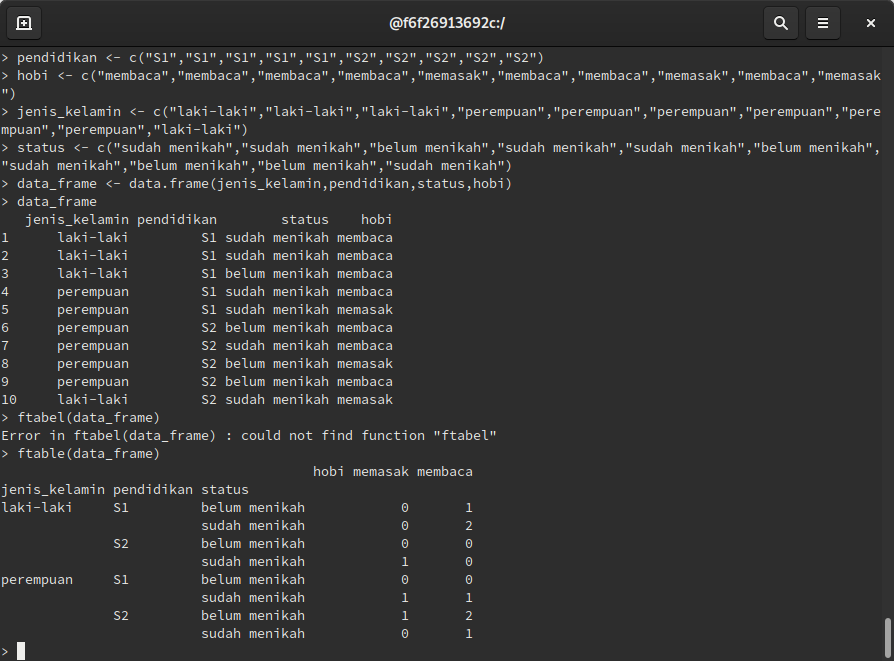
\includegraphics[width=\linewidth]{2}
\subsection{Distribusi Frekuensi}
\subsubsection{Praktik 1}
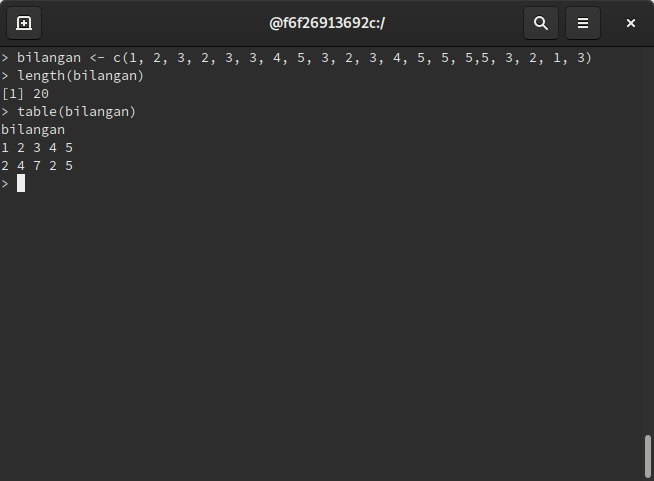
\includegraphics[width=\linewidth]{3}
\subsubsection{Praktik 2}
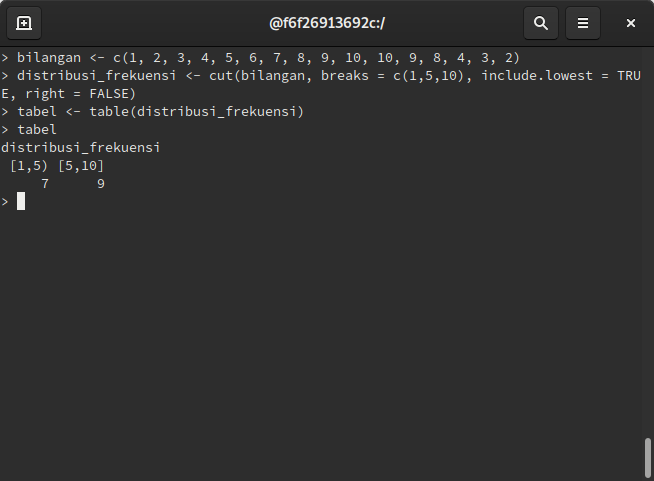
\includegraphics[width=\linewidth]{4}
\section{Latihan}
\subsection{Latihan 1}
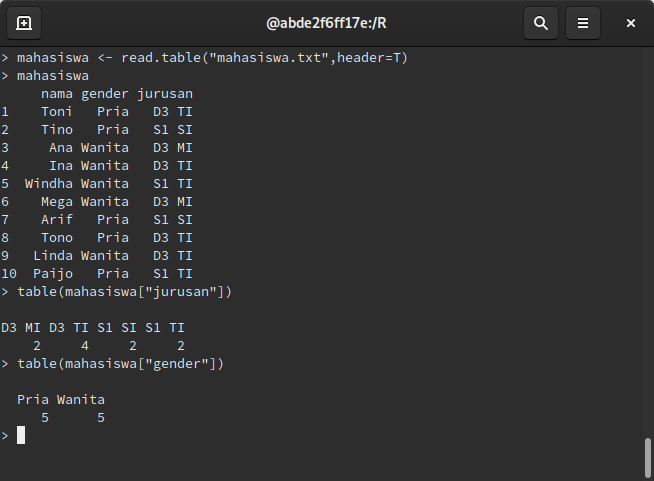
\includegraphics[width=\linewidth]{5}
\subsection{Latihan 2}
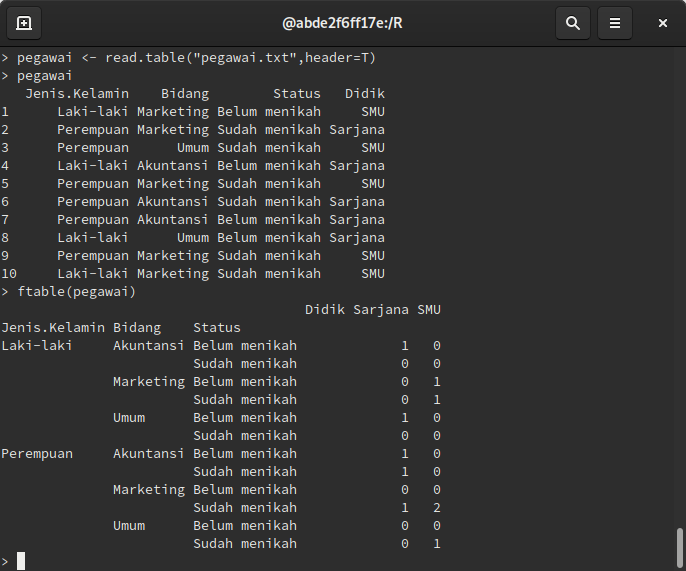
\includegraphics[width=\linewidth]{6}

\end{document}